\documentclass{article}

\usepackage{graphicx}
\usepackage{tikz}
\usepackage{tikzsymbols}
\usetikzlibrary{calc,patterns,shapes.geometric}
\pagestyle{empty}
\usepackage[margin=0pt]{geometry}
\geometry{papersize={14in,12in}}

\def\centerarc[#1](#2)(#3:#4:#5){\draw[#1] ($(#2)+({#5*cos(#3)},{#5*sin(#3)})$) arc (#3:#4:#5);}

\begin{document}
	\begin{figure}
		\centering
		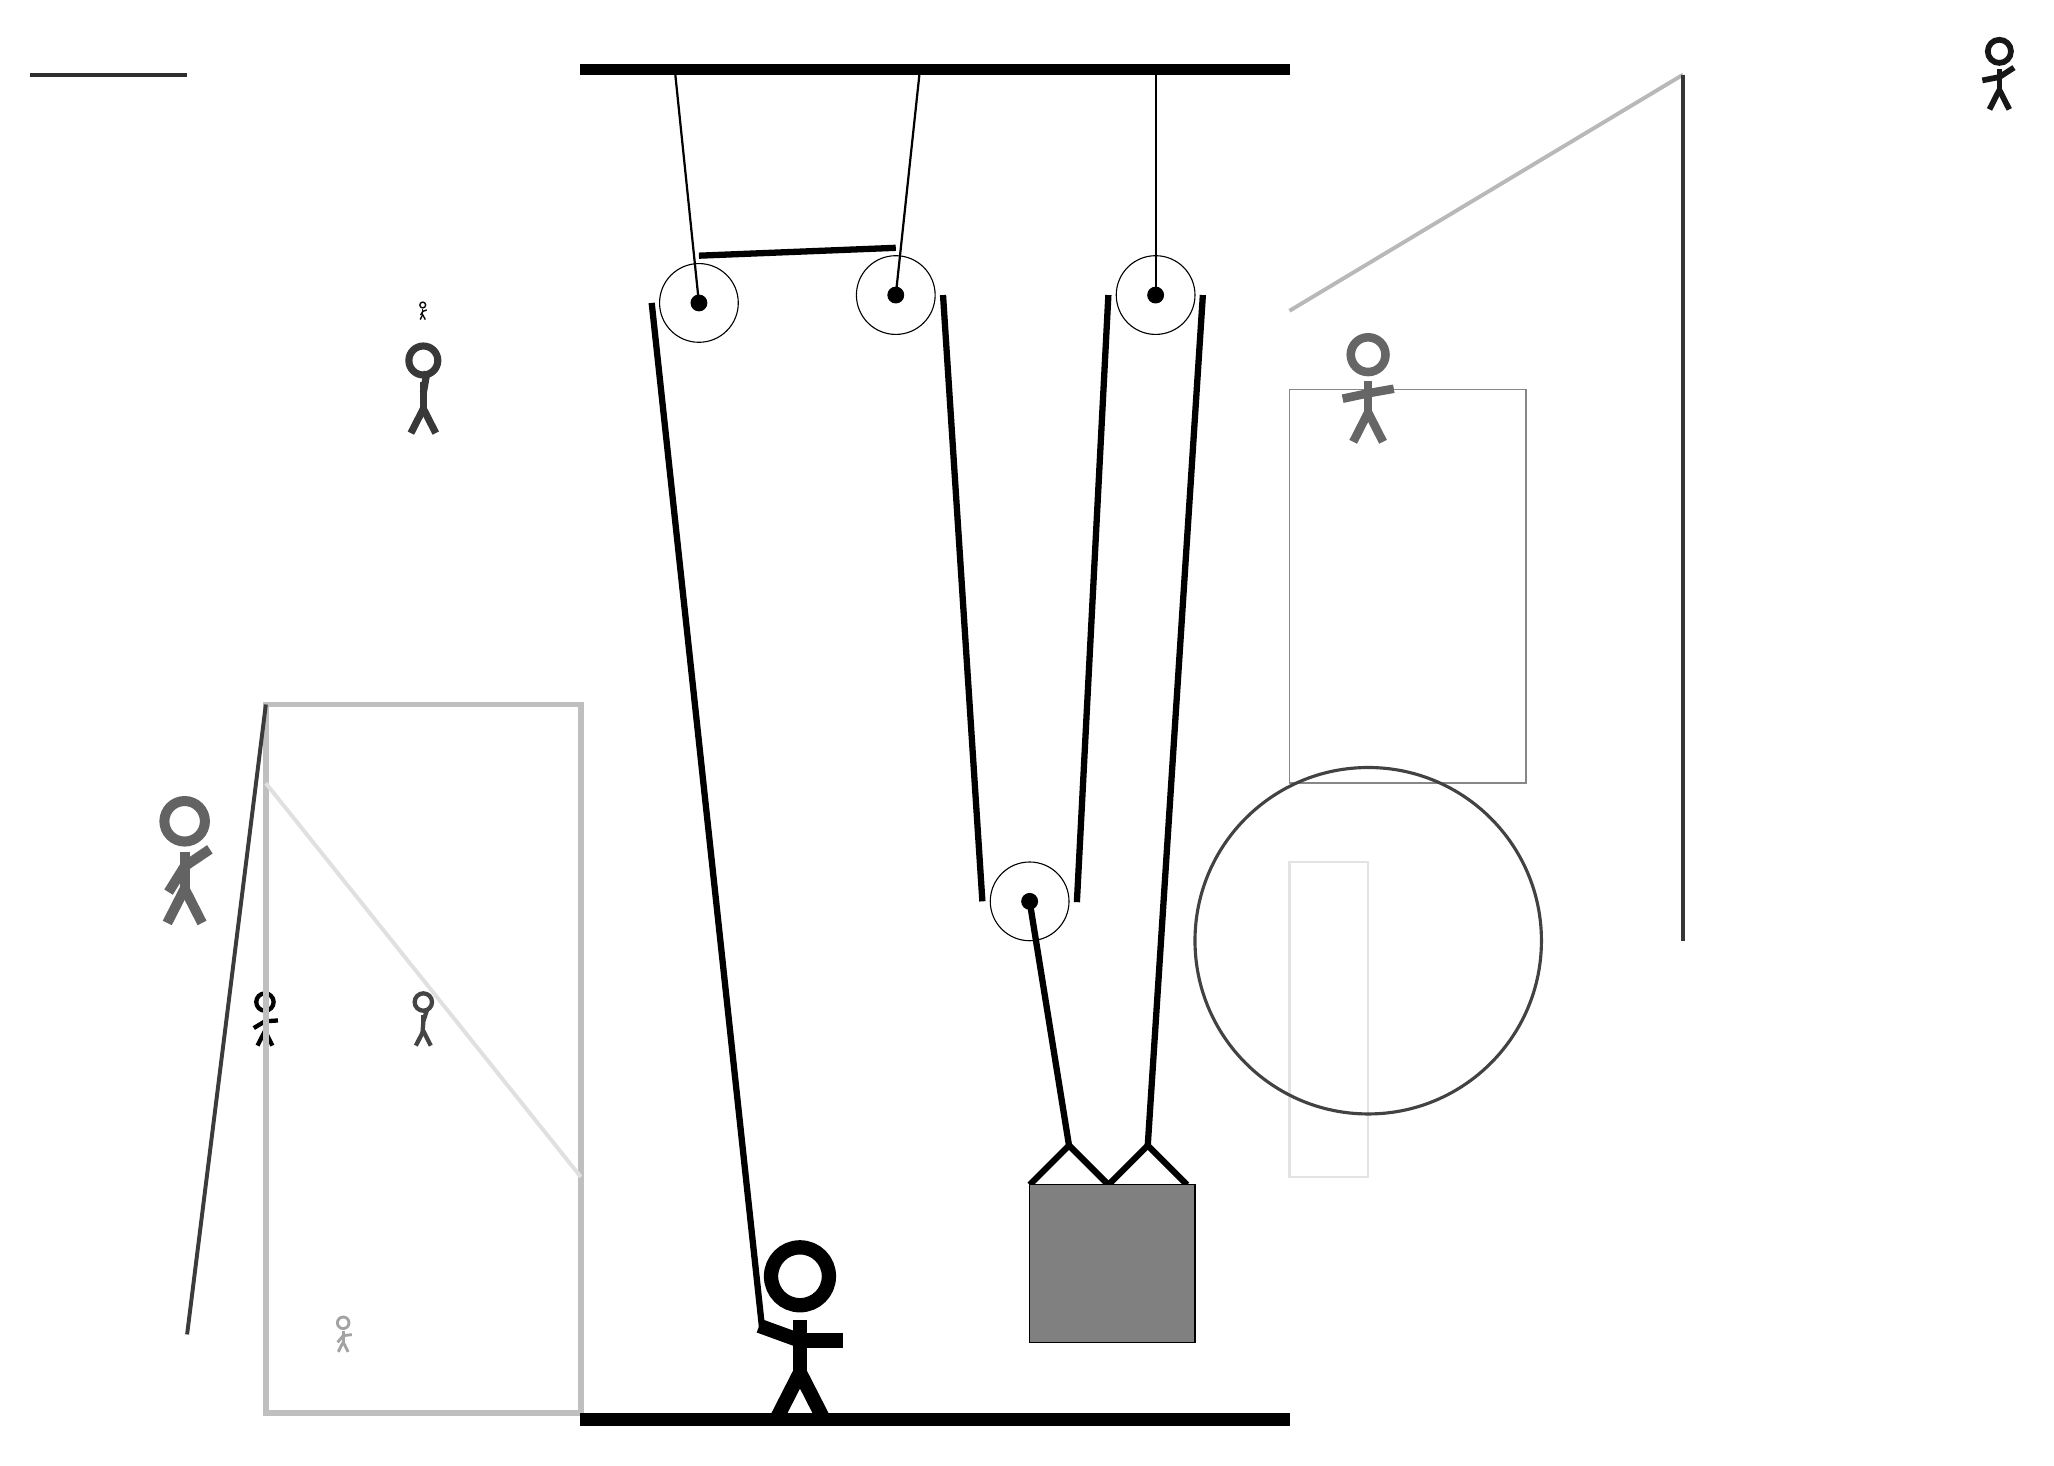
\begin{tikzpicture}
			%%%%% START %%%%%
			
			\draw[fill=black] (-3, 14) rectangle (6, 14.125);
			
			\draw (1, 11.2) circle (0.5);
			\draw[fill=black] (1, 11.2) circle (0.1);
			\draw[thick] (1, 11.2) -- (1.3, 14);
			
			\node[line width=0.6mm, color=black!100] at (-7, 2) {\Strichmaxerl[3][31][4]};
			
			\node[line width=0.2mm, color=black!91] at (15, 14) {\Strichmaxerl[4][11][33]};
			\node[line width=0.6mm, color=black!36] at (-6, -2) {\Strichmaxerl[2][50][7]};
			\draw[line width=0.3mm, color=black!11] (7, 0) rectangle (6, 4);
			\draw[line width=0.5mm, color=black!28](6, 11) -- (11, 14);
			
			\draw[line width=0.2mm, color=black!47] (6, 10) rectangle (9, 5);
			\node[line width=0.4mm, color=black!60] at (7, 10) {\Strichmaxerl[6][12][10]};
			
			\draw[line width=0.7mm, color=black!25] (-3, 6) rectangle (-7, -3);
			\node[line width=0.6mm, color=black!73] at (-5, 2) {\Strichmaxerl[3][86][72]};
			\draw[line width=0.5mm, color=black!77](-8, -2) -- (-7, 6);
			\draw[line width=0.5mm, color=black!79](11, 14) -- (11, 3);
			
			\node[line width=0.7mm, color=black!61] at (-8, 4) {\Strichmaxerl[7][58][34]};
			\draw [line width=0.4mm, color=black!74](7, 3) circle (2.2);
			\node[line width=0.5mm, color=black!78] at (-5, 10) {\Strichmaxerl[5][90][80]};
			\draw[line width=0.5mm, color=black!12](-3, 0) -- (-7, 5);
			\draw[line width=0.5mm, color=black!82](-8, 14) -- (-10, 14);
			\node[line width=0.6mm, color=black!96] at (-5, 11) {\Strichmaxerl[1][60][20]};
			
			
			\draw (4.3, 11.2) circle (0.5);
			\draw[fill=black] (4.3, 11.2) circle (0.1);
			\draw[thick] (4.3, 11.2) -- (4.3, 14);
			
			\draw (2.7, 3.5) circle (0.5);
			\draw[fill=black] (2.7, 3.5) circle (0.1);
			
			\draw[line width=0.8mm]  (2.7, -0.1) -- (3.2, 0.4) -- (3.7, -0.1) -- (4.2, 0.4) -- (4.7, -0.1);
			\draw[fill=black!50] (2.7, -0.1) rectangle (4.8, -2.1);
			
			\draw (-1.5, 11.1) circle (0.5);
			\draw[fill=black] (-1.5, 11.1) circle (0.1);
			\draw[thick] (-1.5, 11.1) -- (-1.8, 14);
			
			\draw[line width=0.8mm](-0.7, -1.9) --  (-2.1, 11.1);
			\centerarc[line width=0.8mm](-1.5, 11.1)(90:180:0.6);
			\draw[line width=0.8mm](-1.5, 11.7) -- (1, 11.8);
			\centerarc[line width=0.8mm](1, 11.2)(0:90:0.6);
			\draw[line width=0.8mm](1.6, 11.2) -- (2.1, 3.5);
			\centerarc[line width=0.8mm](2.7, 3.5)(180:370:0.6);
			\draw[line width=0.8mm] (3.3, 3.49) -- (3.7, 11.2);
			\centerarc[line width=0.8mm](4.3, 11.2)(0:180:0.6);
			\draw[line width=0.8mm](4.2, 0.4) -- (4.9, 11.2);
			\draw[line width=0.8mm] (3.2, 0.4) -- (2.7, 3.5);
			
			\node at (-0.2, -2) {\Strichmaxerl[10][-20][0]};
			
			\draw[fill=black] (-3, -3) rectangle (6, -3.15);
			
			%%%%% END %%%%%
		\end{tikzpicture}
	\end{figure}	
\end{document}